\section{KHR}
\subsection{Mengi (e. Sets)}
Finnum stök í eftirfarndi mengja.\\
a) \{$x | x \in \mathbb{R} \wedge x^2=1 $\} = \{-1,1\}\\
Þar sem öll stök í öðru þurfa að vera jaft og 1 í mengi okkar þá erum við bara með 1 og -1.\\
b) \{$x|x$ er jákvæð heiltala meira en 12\} = \{1,2,3,4,5,6,7,8,9,10,11\} eða \{$1,2,3\ldots ,11$\}\\
c) \{x|x er ferningstala og x < 100\} eða $\sqrt{n}\in \mathbb{Z}$\\
= \{1,4,9,16,25,26,49,64,81\}\\
d)\{x|x er heiltala og $x^2 = 2$\} = \{\} eða tómamengi sem er svona $\varnothing$\\
\\
Annað dæmi.\\
Látum $A=\{a,b,c,d\}$ og $B=\{x,y\}$ vera mengi.\\
Finnum nú faldmengi(Mengjamargfeldi) $A \times B$ og $B \times A$ $(a,b) \in A \times B$\\
a) $A \times B = \{(a,x), (a,y), (b,x), (b,y), (c,x), (c,y), (d,x), (d,y)\}$\\
\indent Það sem þarf að hafa í huga er að þar sem við byrjum með $A$ og svo $\times B$ þá \indent þrufa öll stök í $A$ að vera á undan með öll stök í $B$. Það má lýkja þessu við \indent hnita kerfi þar sem stökin eru púntar á hnita kerfinnu.\\
b) $B \times A = \{(x,a), (x,b), (x,c), (x,d), (y,a), (y,b), (y,c), (y,d)\}$\\
\\
Annað dæmi\\
Ef A hefur m stök og B hefur n mörg stök, hvað eru þó mörg stök í $A \times B$\\
$A \times B$ er þá svona:\\
$(a_1,b_1),(a_2,b_1),(a_3,b_1), \ldots ,(a_m,b_1)
\\ 
(a_1,b_2),(a_2,b_2),(a_3,b_2), \ldots ,(a_m,b_2)
\\
(a_1,b_3),(a_2,b_3),(a_3,b_3), \ldots ,(a_m,b_3)
\\ \vdots \\
(a_1,b_n),(a_2,b_n),(a_3,b_n), \ldots ,(a_m,b_n)$\\
Þannig það er $n*m$ mörg stök í $A \times B$.\\
\newpage
\subsection{Mengjaaðgerðir (e. Set Operations)}
Látum A og B vera mengi.\\
A er mengi: Nemanda sem búa innan við km frá skólanum.\\
B er mengi: Nemaenda sem ganga í skólann.\\
Við ætlum að finna.\\
a) $A\cap B$ er mengi nemanda sem búa nið innan km frá skólanum og ganga í skólann.\\
b) $A \cup B$ er mengi nemanda sem sem búa við innan km við skólann eða ganga í skólann. (allt í báðum mengjum)\\
c) $A - B$ er mengi nemanda sem búa við innan km við skólann en ganga ekki í skólann. (allt sem er inn í A en ekki B og $A \cap B$)\\
d)$B-A$ er mengi nemanda sem búa ekki innan km við skólann en ganga í skólann. (allt sem er inn í B en ekki A og $B \cap A$)\\
\\
Annað dæmi um stóru merginn þar sem við endurtökum rökvirkjan okkar.\\
Látum $A_i = \{1,2,3,\ldots ,i\}$ vera mengi.\\
Þar sem $i \in \mathbb{Z}_+$ Jákvæðar heiltölur.\\
Finnum: Sammengi.\\

a) $\displaystyle \bigcup_{i=1}^n A_i = A_1 \cup A_2 \cup A_3 \cup \ldots \cup A_n$ Það sem $n \in \mathbb{Z}_+$\\

b) $\displaystyle \bigcup_{i=1}^n A_i = A_1 \cup A_2 \cup A_3 \cup \ldots \cup A_n$ Hvernig er þetta þegar við legjum það saman.\\
\begin{align*}
    & \{1\}\\
    \cup & \{1,2\}\\
    \cup & \{1,2,3\}\\
    \cup & \ldots\\
    \cup & \{1,2,3, \ldots ,n\}
\end{align*}

c) $\displaystyle \bigcap_{i=1}^n A_i = A_1 \cap A_2 \cap A_3 \cap \ldots \cap A_n$ Sniðmengi er bara $\{1\}$\\
\begin{align*}
    & \{1\}\\
    \cap & \{1,2\}\\
    \cap & \{1,2,3\}\\
    \cap & \ldots\\
    \cap & \{1,2,3, \ldots ,n\}
\end{align*}
\newpage

\subsubsection{Sanna De morgan law}
Látum A og B vera mengi.\\
Sönnum seinni De Morgan Reglu sem er $\overline{A \cup B} = \overline{A} \cap \overline{B}$\\
a) Notum við "set builder notation" og fáum.
\begin{align*}
    \overline{A \cup B} &= \{x|x \in \overline{A \cup B}\} \quad \text{skv. skilgr. set builder notation} \\
    &= \{x|x \notin A \cup B\} \quad \text{skv. skilgr. fyllimengi} \\
    &= \{x|\lnot (x \in A \cup B)\} \quad \text{skv. skilgr.} \notin \\
    &= \{x|\lnot (x \in A \vee x \in B)\} \quad \text{skv. skilgr. sammengi}\\
    &= \{x|\lnot (x \in A) \wedge \lnot(x \in B)\} \quad \text{skv. De Morgan rökvirkja} \\
    &= \{x| x \notin A \wedge x \notin B\} \quad \text{skv. skilgr.} \notin \\
    &= \{x|x \in \overline{A} \wedge x \in \overline{B}\} \quad \text{skv. skilgr. fyllimengi}\\
    &= \{x|x \in (\overline{A} \cap \overline{B})\} \quad \text{skv. skilgr. sniðmengi}\\
    &= \overline{A} \cap \overline{B} \quad \text{skv. skilgr. set builder notation}
\end{align*}
Af þessu sést að $\overline{A \cup B} = \overline{A} \cap \overline{B}$.\\
\\
b) Notum íverutöflu. Skoðum töfluna.\\ \\
\begin{tabular}{ c|c|c|c|c|c|c }
    A & B & $\overline{A}$ & $\overline{B}$ & $A \cup B$ & $\overline{A \cup B}$ & $\overline{A} \cap \overline{B}$
    \\ \hline
    1 & 1 & 0 & 0 & 1 & 0 & 0 \\
    1 & 0 & 0 & 1 & 1 & 0 & 0 \\
    0 & 1 & 1 & 0 & 1 & 0 & 0 \\
    0 & 0 & 1 & 1 & 0 & 1 & 1
\end{tabular} \vspace*{1em}
\\ 
Við sjáum að stök í $\overline{A \cup B}$ og $\overline{A} \cap \overline{B}$ eru þau sömmu. \\
\newpage

\setcounter{section}{8}
\setcounter{subsection}{4}
\subsection{Talning staka í mengjum (e. Inclusion– Exclusion)}
Látum A og B verqa mengi þar að með sterð á.\\
$|A| = 12$ og $|B| = 18$. Finnum $|A \cup B|$ ef. \quad Formúla $|A \cup B| = |A| + |B| - |A \cap B|$ \\
\indent a) $|A \cap B| = 0$ Við fáum þá $|A \cup B| = |A| + |B| - |A \cap B| = 12 + 18 - 0 = 30$
\begin{center}
    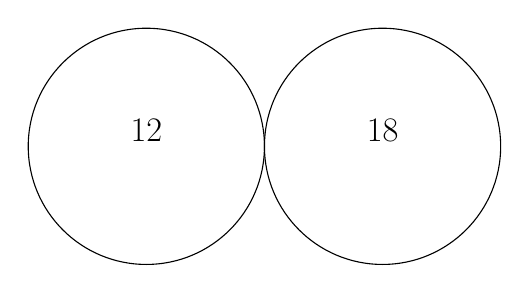
\begin{tikzpicture}[scale=0.5, transform shape]
        \draw (-3,2) circle (3cm) node[above] {\Huge 12};
        \draw (3,2) circle (3cm) node[above] {\Huge 18};
    \end{tikzpicture}
\end{center}
\indent \indent Við sjáum að hringinnir skera ekki saman.\\
\indent b) $|A \cap B| = 1$ Við fáum þá $|A \cup B| = |A| + |B| - |A \cap B| = 12 + 18 - 1 = 29$
\begin{center}
    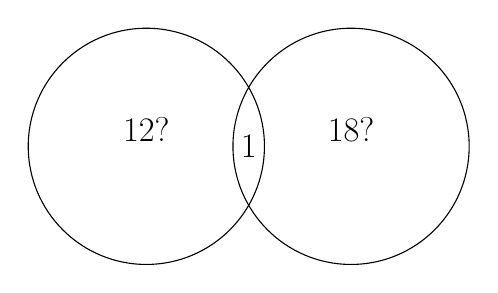
\begin{tikzpicture}[scale=0.5, transform shape]
        \draw (-2.6,2) circle (3cm) node[above] {\Huge 12?};
        \draw (2.6,2) circle (3cm) node[above] {\Huge 18?};
        \node at (0,2) {\Huge 1};
    \end{tikzpicture}
\end{center}
\indent \indent Við situm ? á 12 og 18 þar sem við vitum ekki alveg hvað er í $|A|$ og $|B|$ nema \indent að allt saman er 29.\\
\indent c) $|A \cap B| = 6$ Við fáum þá $|A \cup B| = |A| + |B| - |A \cap B| = 12 + 18 - 6 = 24$
\begin{center}
    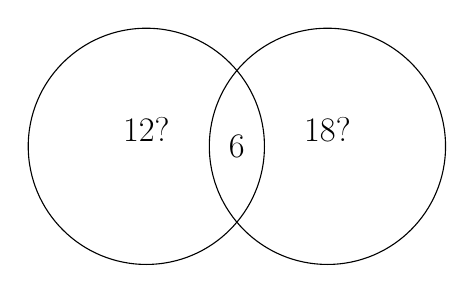
\begin{tikzpicture}[scale=0.5, transform shape]
        \draw (-2.3,2) circle (3cm) node[above] {\Huge 12?};
        \draw (2.3,2) circle (3cm) node[above] {\Huge 18?};
        \node at (0,2) {\Huge 6};
    \end{tikzpicture}
\end{center}
\indent \indent Við situm aftur ? á 12 og 18 þar sem við vitum ekki alveg hvað er í $|A|$ og $|B|$ \indent nema að allt saman er allt 24.\\
\indent d) $A \subseteq B$ ($\subseteq$ = Öll stök í A eru í B). Formúlan ($|A \cap B| = |A| = 12$).\\
Fáum: $|A \cup B| = |A| + |B| - |A \cap B| = 12 + 18 - 12 = 18$
\begin{center}
    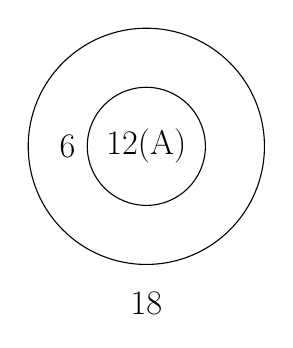
\begin{tikzpicture}[scale=0.5, transform shape]
        \draw (0,2) circle (3cm) node {\Huge 12(A)};
        \draw (0,2) circle (1.5cm);
        \node at (-2,2) {\Huge 6};
        \node at (0,-2) {\Huge 18};
    \end{tikzpicture}
\end{center}
\newpage

\subsubsection{Annað dæmi} 
Látum U vera mengi nemanda, R vvera mengi nemanda sem borða rósakál, S fyrir brokolí og B fyrir blómkál. Regla: $|\overline{A}| = |U| - |A|$\\
Þá vitum við að:
\begin{multicols}{2}
    \hspace*{-1.3em}$|U|=270$ \hspace*{0.5em} $|R \cap S| = 26$\\
    $|R|=64$  \hspace*{1em} $|R \cap B| = 28$\\
    $|S|=94$  \hspace*{1.1em} $|S \cap B| = 22$\\
    $|B|=58$  \hspace*{1em} $|B \cap S \cap B| = 14$
    
    \columnbreak
    \vspace*{-1cm}
    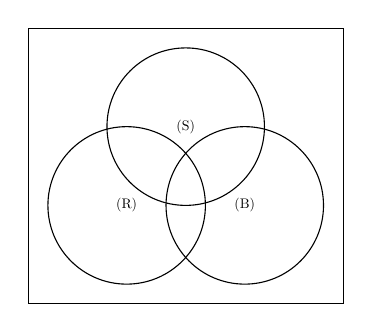
\begin{tikzpicture}[scale=0.5, transform shape]
        \draw (0,0) rectangle (8,7);
        \draw (2.5,2.5) circle (2cm) node {(R)};
        \draw (5.5,2.5) circle (2cm) node {(B)};
        \draw (4,4.5) circle (2cm) node {(S)};
    \end{tikzpicture}
\end{multicols}
\hspace*{-1.3em}Finnum hvessu mergir nemendur borða ekkert þessa grasmetis.\\ 
Formúla til að finna svar:\\ 
$|A \cup B \cup C| = |A| + |B| + |C| - |A \cap B| - |A \cap C| - |B \cap C| + |A \cap B \cap C|$ \\
Við byrjum á að telja allt í A, B og C en þá teljum við líka það sem er á milli þanni við mínusum það en þá vantar okkur það sem skel á milli alla þeira þannig við + það við.\\
$|R \cup S \cup B| = |R| + |S| + |B| - |R \cap S| - |R \cap B| - |S \cap B| + |R \cap S \cap B|$ =\\
$64 + 94 + 58 - 26 - 28 - 22 + 14 = 154$ Sem borða eitthvað grameti.\\
Þá fæst að $|\overline{R \cup S \cup B}| = |U| - |R \cup S \cup B| = |R| + |S| + |B| - |R \cap S| - |R \cap B| - |S \cap B| + |R \cap S \cap B|$ eða $270 - 154 = 116$ Sem eru fyrir utan.
\newpage

\setcounter{section}{2}
\setcounter{subsection}{2}
\subsection{Föll (e. Functions)}
Ákveðum ef F er fall út frá bitastrengja í mengi heiltölu.\\
\hspace*{1em}a) F(s) er sæti núllbits í S.\\
\hspace*{1em}F er ekki fall því F(00) hefur tvær mismunandi útkomur þá 1,2\\
\hspace*{1em}b) F(s) er fjöldi ása í S. \\
\hspace*{1em}Við sjáum að þetta er fall þar sem við getum gert $F(1) = 1$, $F(110) = 2$, \hspace*{1em}$F(0) = 0$. Við skilum alltaf einni útkomu.\\
\hspace*{1em}F(s) er minsta heiltalan í þar að i-ti bita í S ás og F(s) = 0 ef S er tómastrengur.\\
\hspace*{1em}F er ekki fall því það er ekki skilgrent fallgildi ef S innheldur bara 0.\\

\subsubsection{Loft föll og gólf föll}
Finnum eftirfarndi gildi:\\
\hspace*{1em}a) $\lceil - \frac{3}{4} \rceil = 0$. Loft föll fara alltaf upp líka þegar við erum fyrir neðan 0.\\
\hspace*{1em}b) $\lfloor - \frac{7}{8} \rfloor = -1$ Gólf fall fer alltaf niður.\\
\hspace*{1em}c) $\lfloor \frac{1}{2} + \lceil \frac{3}{2} \rceil  \rfloor = \lfloor \frac{1}{2} + 2 \rfloor = \lfloor 5/2 \rfloor = 2$ Loft og gólf föll virka eins og svigar þar \hspace*{1em}sem við byrjum á insta og vinnum okkur út.\\
\newpage

\subsection*{Lögar og vísar}
\subsubsection*{Veldis reglur}
Reglur: $a^m * a^n = a^{m+n}$ \quad $(a^m)^n = a^{m*n}$ \quad $^n\sqrt{a} = a^{1/n}$\\
a) Svona er dæmið: $2*2^2$ en veð horfum á þetta svona $2^1*2^2 = 2^{1+2} = 2^3$\\
b) $(2^2)^3 = 2^{2*3} = 2^6$\\
c) $2^{2^2} = 2^4$
\subsubsection*{Log}
Finnum eftirfarndi stærðir \quad Regla: $\log_a(a^m)=m$\\
a) $\log_2(1024) = \log_2(2^{10}) = 10$ þar sem $2^{10}$ er 1024.\\
b) $\log_2(1/4 = \log_2((1/2)^2)) = \log_2(2^{-2}) = -2$\\
c) $\log_4(8) = \log_4(2^3) = \log_4((4^{1/2})^3) = \log_4(4^{3/2}) = 3/2$
\newpage

\subsection{Runur og summur (e. Sequences and Summations)}
Látum $\{a_n\}$ vera runu þar sem liðurinn $a_n = 2* (-3)^n + 5^n$\\
a) $a_0 = 2* (-3)^0 + 5^0 = 2*1+1=3$\\
b) $a_1 = 2* (-3)^1 + 5^1 = 2 * (-3)+5=-1$\\
b) $a_4 = 2* (-3)^4 + 5^4 = 2 * 81 + 625 = 787$\\
b) $a_5 = 2* (-3)^5 + 5^5 = 2 * (-243) + 3125 = 2639$\\
Það er líka hægt að vera með runur svona.\\
Rúna sem byrjar á 2 og hver liður hæklar um 3\\
\hspace*{1em}2,5,8,11,14 \ldots $\infty$\\
\subsubsection{Runur með Reiknisformúlur}
Finnum fyrstu fimm liðina með reiknisformúluni\\
$a_n = a_{n-1}+3*a_{n-2}$ þar sem $a_0 = 1$ og $a_1=2$\\
$a_0 = 1$\\
$a_1 = 2$\\
$a_2 = a_1 +3 * a_0 = 2 + 3 * 1 = 5$\\
$a_3 = a_2 +3 * a_1 = 5 + 3 * 2 = 11$\\
$a_4 = a_3 +3 * a_2 = 11 + 3 * 5 = 26$\\
$a_5 = a_4 +3 * a_3 = 26 + 3 * 11 = 59$\\
\subsubsection{Summur}
Finnum summuna á $\displaystyle \sum_{k=1}^{5} (k+1)$\\
$\displaystyle \sum_{k=1}^{5} (1+1) + (2+1) + (3+1) + (4+1) +(5+1) = 2 + 3 + 4 + 5 + 6 = 20$\\ \\
Finnum tvöfalda summu\\ \\
$\displaystyle \sum_{i=0}^{2} \left(\sum_{j=1}^{3}(ij)\right)$ getur líka verið $\displaystyle \sum_{i=0}^{2} \left(i * \sum_{j=1}^{3}i\right) = \sum_{i=0}^{2}(i(1+2+3))= \sum_{i=0}^{2} (i*6)$\\
Þá erum við með: $\displaystyle 6* \sum_{i=0}^{2}i = 6 * (0 + 1 + 2) = 6 * 3 = 18$
\newpage

\setcounter{subsection}{5}
\subsection{Fylki (e.Matrices)}
Regla: Telja Lína x Dálkur.\\ 
\\
Skoðum fylkið A =
$\begin{bmatrix}
    1 & 1 & 1 & 3 \\
    2 & 0 & 4 & 6 \\
    1 & 1 & 3 & 7 \\
\end{bmatrix}$\\
\\
a) Hver er stærð á fylkinu: Það er $3x4$ að stærð.\\
\\
b) Hver er þryðji dálkur í fylkinu: $3x1$ eða = 
$\begin{bmatrix}
    1 \\
    4 \\
    3
\end{bmatrix}$\\
\\
c) Önnur lína fylkisins er: $1x4$ fylkið =
$\begin{bmatrix}
    2 & 0 & 4 & 6
\end{bmatrix}$\\
\\
d) Hvaða stak er númer (3,2) eða stakið í sæti: 1 (þetta er ekki fylki heldur stak.).\\
\\
e) Finnum bylt fylkið $A^T$ er fylkið: A fyrkið verður 4x3: 
$\begin{bmatrix}
    1 & 2 & 1 \\
    1 & 0 & 1 \\
    1 & 4 & 3 \\
    3 & 6 & 7
\end{bmatrix}$

\vspace*{-1.6em}
\subsubsection{Margföldun Fylkja} 
Finnum AB ef: \quad Regla: $(k * m) * (m * n) = k*n$\\
\\
a) A = 
$\begin{bmatrix}
    2 & 1 \\
    3 & 2
\end{bmatrix}$ og B = 
$\begin{bmatrix}
    0 & 4 \\
    1 & 3    
\end{bmatrix}$ Fáum: AB = 
$\begin{bmatrix}
    2 & 1 \\
    3 & 2
\end{bmatrix} 
\begin{bmatrix}
    0 & 4 \\
    1 & 3    
\end{bmatrix}$ = 
$\begin{bmatrix}
    2*0 + 1*1 & 2*4 + 1*3  \\
    3*0 + 2*1 & 3*4 + 2*3
\end{bmatrix}$\vspace*{0.7em} =
$\begin{bmatrix}
    0 + 1 & 8 + 3  \\
    0 + 2 & 12 + 6
\end{bmatrix}$ =
$\begin{bmatrix}
    1 & 11 \\
    2 & 18
\end{bmatrix}$\\ \\
b) A =
$\begin{bmatrix}
    1 & -1 \\
    0 & 1 \\
    2 & 3
\end{bmatrix}$ og B = 
$\begin{bmatrix}
    3 & -2 & -1 \\
    1 & 0 & 2    
\end{bmatrix}$ AB = 
$\begin{bmatrix}
    1 & -1 \\
    0 & 1 \\
    2 & 3
\end{bmatrix}$
$\begin{bmatrix}
    3 & -2 & -1 \\
    1 & 0 & 2    
\end{bmatrix}$\vspace*{0.7em} \\ =  
$\begin{bmatrix}
    1*3 + (-1)*1 & 1*(-2) + (-1)*0 & 1*(-1) + (-1)*2 \\
    0*3 + 1*1 & 0*(-2) + 1*0 & 0*(-1) + 1*2 \\
    2*3 + 3*1 & 2*(-2) + 3*0 & 2*(-1) + 3*2 \\
\end{bmatrix}$ \vspace*{0.7em} \\ =  
$\begin{bmatrix}
    3 + -1 & -2 + 0 & -1 + -2 \\
    0+1 & 0+0 & 0+2 \\
    6+3 & -4+0 & -2+6
\end{bmatrix}$ = 
$\begin{bmatrix}
    2 & -2 & -3 \\
    1 & 0 & 2 \\
    0 & -4 & 4
\end{bmatrix}$
\newpage
\subsubsection{Fylkja graf og stærð}
Hvað vitum við um fylki A og B ef margfeldi AB og BA eru skilgreind?\\
Margfeldi AB er aðeins skilgreind ef A hefur jafnmarga dálka og B hefur línur.\\
Ef A af stærð $n \times m$ og B af stærð $s \times t$ gildir þýðir það að m = s.\\
Á hliðstæðan hátt fæst að BA er skilgreind aðeins ef n = t.\\
Þannig að ef A er $n \times m$ að stærð þá er B $m \times n$ að stærð.\\
A = 
$\begin{bmatrix}
    1 \\
    2 \\
    3 \\
    4
\end{bmatrix}$ B = 
$\begin{bmatrix}
    1 & 2 & 3 & 4
\end{bmatrix}$

\subsubsection{Hornlínufylki}
Hornlínufylki er fylki þar sem öll stök eru 0 nema á hornalínu.\\
Sýnum að margfeldi tveggja hornalínufylki er hornalínufylki.\\
Látum A og B vera hornalínufylki af stærð $n \times n$. \vspace*{1em}\\
A = 
$\begin{bmatrix}
    a_{1,1} & 0 & 0 & \cdots & 0 \\
    0 & a_{2,2} & 0 & \cdots & 0 \\
    0 & 0 & a_{3,3} & \cdots & 0 \\
    \vdots & \vdots & \vdots & \ddots & \vdots \\
    0 & 0 & 0 & \cdots & a_{n,n} \\
\end{bmatrix}$ B =
$\begin{bmatrix}
    b_{1,1} & 0 & 0 & \cdots & 0 \\
    0 & b_{2,2} & 0 & \cdots & 0 \\
    0 & 0 & b_{3,3} & \cdots & 0 \\
    \vdots & \vdots & \vdots & \ddots & \vdots \\
    0 & 0 & 0 & \cdots & b_{n,n} \\
\end{bmatrix}$ \vspace*{1em} \\
Skoðum nú AB. Þegar lína i er margfölduð við dálk i fæst:\\ 
$0+0+\ldots+a_{i,i}+b_{i,i} = a_{i,i},b_{i,i}$.\\
Þannig að stak í $c_{i,i}$ í AB er ekki endilega 0.\\
Skoðum nú stak $c_{i,j}$ þar sem $i \not = j$. Við Margföldun línu i í A við dálk j í B.\\
Þá fæst að $c_{i,j} = 0+0+\ldots+a_{i,i}\times0+b_{j,j}\times0+\ldots+0=0$. Því $i \not = j$.\\
\newpage

\subsubsection{Fylkja formúlur}
Látum A = 
$\begin{bmatrix}
    1 & 1 \\
    0 & 1
\end{bmatrix}$ vera fylki.\\
Finnum formúlu fyrir $A^n$ þar sem $n \in \mathbb{Z}_+$\vspace*{1em} \\
$A^1 = A = 
\begin{bmatrix}
    1 & 1 \\
    0 & 1
\end{bmatrix}$\\
$A^2 = AA = 
\begin{bmatrix}
    1 & 1 \\
    0 & 1
\end{bmatrix}
\begin{bmatrix}
    1 & 1 \\
    0 & 1
\end{bmatrix} = 
\begin{bmatrix}
    1 & 2 \\
    0 & 1
\end{bmatrix}$\\
$A^3 = A^2A = 
\begin{bmatrix}
    1 & 2 \\
    0 & 1
\end{bmatrix}
\begin{bmatrix}
    1 & 1 \\
    0 & 1
\end{bmatrix} = 
\begin{bmatrix}
    1 & 3 \\
    0 & 1
\end{bmatrix}$\\
$A^4 = A^3A = 
\begin{bmatrix}
    1 & 4 \\
    0 & 1
\end{bmatrix}
\begin{bmatrix}
    1 & 1 \\
    0 & 1
\end{bmatrix} = 
\begin{bmatrix}
    1 & 4 \\
    0 & 1
\end{bmatrix}$\vspace*{1em}\\
Sem segir okkur að formúlan fyrir $A^n$ =
$\begin{bmatrix}
    1 & n \\
    0 & 1
\end{bmatrix}$ \vspace*{1em} \\
Vegna þessa að $a_{1,2}$ er einna stakið sem er ekki markfaldað með 0.

\subsubsection{Anndhverfa filkis.}
Látum A = $\begin{bmatrix}
    a & b \\
    c & d 
\end{bmatrix}$ vera fylki\vspace*{1em} \\
Sýnum að ef $ad-bc \not = 0$ þá er: $A^{-1} = 
\begin{bmatrix}
    \frac{d}{ad-bc} & \frac{-b}{ad-bc} \\
    \frac{-c}{ad-bc} & \frac{a}{ad-bc} 
\end{bmatrix}$\vspace*{1em} \\
Ef AB = I og BA = I þá er $A^{-1} = B$. Þar sem $I_3$ = 
$\begin{bmatrix}
    1 & 0 & 0 \\
    0 & 1 & 0 \\ 
    0 & 0 & 1
\end{bmatrix}$ eða hornalínufylki.\vspace*{1em}\\
$\begin{bmatrix}
    a & b \\
    c & d 
\end{bmatrix}
\begin{bmatrix}
    \frac{d}{ad-bc} & \frac{-b}{ad-bc} \\
    \frac{-c}{ad-bc} & \frac{a}{ad-bc} 
\end{bmatrix}$ = 
$\begin{bmatrix}
    \frac{ad}{ad-bc} - \frac{bc}{ad-bc} & \frac{-ab}{ad-bc} - \frac{ab}{ad-bc}\vspace*{0.5em} \\
    \frac{cd}{ad-bc} - \frac{cd}{ad-bc} & \frac{-bc}{ad-bc} - \frac{da}{ad-bc}
\end{bmatrix}
\begin{bmatrix}
    \frac{ab-bc}{ad-bc} & \frac{ab-ab}{ad-bc}\vspace*{0.5em} \\
    \frac{cd-cd}{ad-bc} & \frac{cd-bc}{ad-bc}
\end{bmatrix}
\begin{bmatrix}
    1 & 0 \\
    0 & 1 \\
\end{bmatrix}$\vspace*{1em} \\
$\begin{bmatrix}
    \frac{d}{x} & \frac{-b}{x}\vspace*{0.2em} \\
    \frac{-c}{x} & \frac{a}{x} \\
\end{bmatrix}
\begin{bmatrix}
    a & b \\
    c & d \\
\end{bmatrix} = 
\begin{bmatrix}
    1 & 0 \\
    0 & 1 \\
\end{bmatrix}$ Reiknað eins og hitt.\\

\newpage
\subsubsection{Rökvirkja fylki}
Látum A = 
$\begin{bmatrix}
    1 & 0 & 1 \\
    1 & 1 & 0 \\
    0 & 0 & 1 \\
\end{bmatrix}$ og B = 
$\begin{bmatrix}
    0 & 1 & 1 \\
    1 & 0 & 1 \\
    1 & 0 & 1 \\
\end{bmatrix}$ vera bitafylki.\vspace*{1em}\\
a) Finnum $A \vee B$ = 
$\begin{bmatrix}
    1 & 0 & 1 \\
    1 & 1 & 0 \\
    0 & 0 & 1 \\
\end{bmatrix}\vee 
\begin{bmatrix}
    0 & 1 & 1 \\
    1 & 0 & 1 \\
    1 & 0 & 1 \\
\end{bmatrix} = 
\begin{bmatrix}
    1 & 1 & 1 \\
    1 & 1 & 1 \\
    1 & 0 & 1 \\
\end{bmatrix}$\vspace*{1em} \\
b) Finnum $A \wedge B$ =
$\begin{bmatrix}
    1 & 0 & 1 \\
    1 & 1 & 0 \\
    0 & 0 & 1 \\
\end{bmatrix}\wedge 
\begin{bmatrix}
    0 & 1 & 1 \\
    1 & 0 & 1 \\
    1 & 0 & 1 \\
\end{bmatrix} = 
\begin{bmatrix}
    0 & 0 & 1 \\
    1 & 0 & 0 \\
    0 & 0 & 1 \\
\end{bmatrix}$\vspace*{1em} \\
c) Finnum $A \odot B$ =
$\begin{bmatrix}
    1 & 0 & 1 \\
    1 & 1 & 0 \\
    0 & 0 & 1 \\
\end{bmatrix}\odot
\begin{bmatrix} 
    0 & 1 & 1 \\
    1 & 0 & 1 \\
    1 & 0 & 1 \\
\end{bmatrix}\vspace*{0.5em} \\
\begin{bmatrix}
    (1\wedge0) \vee (0\wedge1) \vee (1\wedge1) & (1\wedge1) \vee (0\wedge0) \vee (1\wedge0) & (1\wedge1) \vee (0\wedge1) \vee (1\wedge1) \\
    (1\wedge0) \vee (1\wedge1) \vee (0\wedge1) & (1\wedge1) \vee (1\wedge0) \vee (0\wedge0) & (1\wedge1) \vee (1\wedge1) \vee (0\wedge1) \\
    (0\wedge0) \vee (0\wedge1) \vee (1\wedge1) & (0\wedge1) \vee (0\wedge0) \vee (1\wedge0) & (0\wedge1) \vee (0\wedge1) \vee (1\wedge1) \\
\end{bmatrix}\vspace*{0.5em} \\ = 
\begin{bmatrix} 
    1 & 1 & 1 \\
    1 & 1 & 1 \\
    1 & 0 & 1 \\
\end{bmatrix}$

\subsubsection*{Með veldi}

Látum A = 
$\begin{bmatrix}
    1 & 0 & 0 \\
    1 & 0 & 1 \\
    0 & 1 & 0 \\
\end{bmatrix}$ vera bitafylki.\\
a) Fáum $A^{[2]}= A \odot A = 
\begin{bmatrix}
    1 & 0 & 0 \\
    1 & 1 & 0 \\
    1 & 0 & 1 \\
\end{bmatrix}$ Við stitum okkur leið en á prófi þá þarf að\vspace*{-1.3em} \hspace*{16.7em}sína útreikninga eins og fyrir ofan.\vspace*{1.3em}\\
b) Finnum $A^{[3]}= A^{[2]} \odot A = 
\begin{bmatrix}
    1 & 0 & 0 \\
    1 & 0 & 1 \\
    1 & 1 & 0 \\
\end{bmatrix}$\vspace*{1em}\\
c) Finnum $A \vee A^{[2]} \vee A^{[3]} = 
\begin{bmatrix}
    1 & 0 & 0 \\
    1 & 1 & 1 \\
    1 & 1 & 1 \\
\end{bmatrix}$
\newpage